\chapter{Methodology}
\label{chapter:methodology}
This chapter provides a more detailed explanation of the pipeline previously introduced in Chapter \ref{chapter:proposed_approach}, specifically elucidating the steps leading to our three main objectives: algorithm clasification with WDG, clustering stabilization and ML classification.


\section{Graph-based Framework}
\label{sec:graph_method}
From the \textit{reduced marker set}, obtained after the reduction from the \textit{full marker set} which has been discussed previously, we model the human skeleton as an undirected graph, where the vertices are the joints and the edges represent connections between consecutive physical body joints.\\
Each edge is associated with a specific weight, the value of which depends on a feature extracted from motion capture data. \\
From this \textit{graph skeletal structure}, we define a mathematical game in which the vertices are the players and the edges model the communication channels (through which movement can propagate) between these players. \\
In figure we can see the \textit{graph skeletal structure} without and a table with the joints' labels.
For simplicity, the links are without weights.

\begin{figure}[H]
  \centering
  \begin{subfigure}[b]{0.7\linewidth}
    \centering
    \begin{tikzpicture}
      \node[circle, draw, minimum size=0.8cm] (1) at (1, 0) [] {1};
      \node[circle, draw, minimum size=0.8cm] (2) at (9, 0) [] {2};
      \node[circle, draw, minimum size=0.8cm] (3) at (2.5, 0.9375) [] {3};
      \node[circle, draw, minimum size=0.8cm] (4) at (7.5, 0.9375) [] {4};
      \node[circle, draw, minimum size=0.8cm] (5) at (3, 2.8125) [] {5};
      \node[circle, draw, minimum size=0.8cm] (6) at (7, 2.8125) [] {6};
      \node[circle, draw, minimum size=0.8cm] (7) at (3.5, 5) [] {7};
      \node[circle, draw, minimum size=0.8cm] (8) at (5, 6.25) [] {8};
      \node[circle, draw, minimum size=0.8cm] (9) at (6.5, 5) [] {9};
      \node[circle, draw, minimum size=0.8cm] (10) at (5,8) [] {10};
      \node[circle, draw, minimum size=0.8cm] (11) at (0.7, 7.1875) [] {11};
      \node[circle, draw, minimum size=0.8cm] (12) at (9.3, 7.1875) [] {12};
      \node[circle, draw, minimum size=0.8cm] (13) at (1.7, 7.4) [] {13};
      \node[circle, draw, minimum size=0.8cm] (14) at (8.3, 7.4) [] {14};
      \node[circle, draw, minimum size=0.8cm] (15) at (2.7, 8.6) [] {15};
      \node[circle, draw, minimum size=0.8cm] (16) at (7.3, 8.6) [] {16};
      \node[circle, draw, minimum size=0.8cm] (17) at (3, 10.5) [] {17};
      \node[circle, draw, minimum size=0.8cm] (18) at (5, 10.8375) [] {18};
      \node[circle, draw, minimum size=0.8cm] (19) at (7, 10.5) [] {19};
      \node[circle, draw, minimum size=0.8cm] (20) at (5, 12.5) [] {20};
      
      \foreach \source/\dest/\label/\xshiftval in {20/18//0, 18/17//0, 18/19//0, 17/15//0, 15/13//0, 13/11//0, 19/16//0, 16/14//0, 14/12//0, 18/10//0, 10/8//0, 8/7//0, 7/5//0, 5/3//0, 3/1//0, 8/9//0, 9/6//0, 6/4//0, 4/2//0}
        \path (\source) edge node[xshift=\xshiftval] {\label} (\dest);
    \end{tikzpicture}    
  \end{subfigure}
  \label{fig:graph_skeletal}
  \begin{subfigure}[b]{0.29\linewidth}
    \centering
    \begin{table}[H]
      \centering
      \begin{tabular}{||c||c||}
        \hline
        \textbf{Node} & \textbf{Label} \\
        \hline
        1 & right\_foot \\
        2 & left\_foot \\
        3 & right\_ankle \\
        4 & left\_ankle \\
        5 & right\_knee \\
        6 & left\_knee \\
        7 & right\_hip \\
        8 & hip\_center \\
        9 & left\_hip \\
        10 & spine \\
        11 & right\_hand \\
        12 & left\_hand \\
        13 & right\_wrist \\
        14 & left\_wrist \\
        15 & right\_elbow \\
        16 & left\_elbow \\
        17 & right\_shoulder \\
        18 & shoulder\_center \\
        19 & left\_shoulder \\
        20 & head \\
        \hline
      \end{tabular}
    \end{table}
  \end{subfigure}
  \caption{Skeletal structure and nodes names}
  \label{tab:labels_joints}
\end{figure}



\subsection{Movement features extraction}
\label{subsec:alg_features}
The low-level features extracted for our purpose are \textit{speed}, \textit{tangential acceleration}, and \textit{angular momentum}. \\
While speed indicates how quickly an object is moving, acceleration indicates how rapidly its velocity is changing.
Angular momentum provides information about the rotation of an object around a fixed point.
By incorporating all three quantities as features, a more comprehensive and detailed view of the overall motion is obtained.

\paragraph{Average Velocity} is calculated by finding the change in positions with respect to the delta time, which is the sampling time of the MoCap system and then applying a moving average to obtain a more accurate estimate that is less affected by noise.
We calculate this speed as the norm of the velocity vector.
\begin{equation}
  \vec{v}(t) = \frac{\Delta\vec{r}}{\Delta  t} = \left(\frac{\Delta x}{\Delta t}, \frac{\Delta  y}{\Delta t}, \frac{\Delta z}{\Delta t}\right)
\end{equation}
The final feature consists of the magnitude of the average velocity.

\paragraph{Tangential Acceleration} is obtained in the same way as the average velocity.
\begin{equation}
  \vec{a}(t) = \frac{\Delta\vec{v}}{\Delta t}
\end{equation}

\subsection{Timeseries Smoothing}
After computing the features, we implement two smoothing techniques on the time series data. \\
Firstly, we apply a \textit{Median Filtering} algorithm centered in the middle of the window with $k_1 = 5$. 
On the resulting vector we apply the \textit{Rolling Mean} again centered in the middle of the window with $k_2 = 25 $. \\
Formally with respect to the Formula \ref{eq:rolling_mean}, centering the window means:
\begin{equation}
  rolling(x_i,k) = \frac{1}{k} \sum_{j=i-(k-1)/2}^{i+(k-1)/2} x_j
\end{equation}

The two final features are obtained by applying this procedure and then extracting the magnitude.

\paragraph{Angular Momentum} has been calculated with respect to the center of mass in this way:
\begin{enumerate}
  \item The relative position with respect to the center of mass as: 
  \begin{table}[h]
    \begin{align}
        \vec{s}_{CM} &= \frac{{\sum_{j=1}^{20} \vec{s}_{j}}}{{20}} &
        \vec{s}_{r} &= \vec{s} - \vec{s}_{CM} \label{eq:rel_pos}
    \end{align}
  \end{table}
  \item The relative velocity:
  \begin{table}[H]
    \begin{align}
        \vec{v}_{CM} &= \frac{\vec{ds}_{CM}}{dt} &
        \vec{v}_{r} &= \vec{v} - \vec{v}_{\text{CM}} \label{eq:rel_vel}
    \end{align}
  \end{table}
  \item Lastly the angular momentum relative to the center of mass:
  \begin{table}[H]
    \begin{align}
      \vec{L} = \vec{s}_{r} \times (\vec{v}_{r} \cdot m) \quad with \ m = 1 \ for \ every \ joint \label{eq:ang_mom}
    \end{align}
  \end{table}
\end{enumerate}

Analyzing angular momentum can reveal specific patterns of rotation or changes in orientation.
These patterns can be used to identify distinctive gestures or movements in activities such as gymnastics or choreography.

\paragraph{Similarity measure}
To calculate the weights of the edges connecting the different joints, we utilized \textit{Cosine similarity} as a better similarity measure compared to the one presented in the previous work, after testing its higher performance.
However, since it returns a value between -1 and 1, we added 1 to shift the values and obtain positive weights.
By doing this, it is possible to compare the directions of the two considered nodes, and thus evaluate if two nodes are associated with (nearly) the same direction. \\ 
After obtaining the weights for each edge of the graph, we then have, for each instantaneous frame, a graph $G$ := ($V$, $E$, $w$), where   
$V$ is the set of $vertices$, $E$ is the set of $edges$ and $w$ is the set of $edge weights$.

\subsection{Spectral Clustering}
\label{sec:spectral_clustering}
Clusterization aims to identify groups of nodes that exhibit significant similarity based on the features or data they represent.
This technique is often employed when data is represented as vectors and you want to uncover similarity relationships among these vectors.\\
The Shi-Malik algorithm is a clustering technique based on analyzing the eigenvalues and eigenvectors of the Laplacian matrix of a graph constructed from data.\\
This type of algorithm can be used to partition data into clusters based on their connectivity structure.
Clusterization works to find natural divisions in the graph so that nodes within each cluster are similar to each other based on cosine similarity. \\
The objective is to unveil hidden structures within data so that similar objects are grouped together to aid in data understanding and analysis.
The algorithm has some limitations due to the initialization phase, such as sensitivity to the initial choice of centroids and the requirement to specify the number of clusters beforehand.\\
This is why there will be a subsequent phase of cluster stabilization over time.

\paragraph{Shi-Malik Algorithm} The algorithm can be summarized in these 8 steps:

\begin{enumerate}
    
  \item \textbf{Calculation of Laplacian Matrix:}
  The Laplacian matrix is the difference between the diagonal matrix of node degrees \(D\) and the similarity matrix \(A\):
  \begin{equation}
    L = D - A
  \end{equation}
  
  \item \textbf{Calculation of Laplacian's Eigenvectors and Eigenvalues:}
  Eigenvectors and eigenvalues of the Laplacian matrix are calculated using the $\texttt{np.linalg.eig()}$ function. Eigenvectors represent new transformed data features in the eigenvector space, while eigenvalues provide information about the overall variance of data along the corresponding eigenvectors.
  
  \item \textbf{Selection of Eigenvector to use:}
  Eigenvectors are ordered based on their associated eigenvalues.
  The eigenvector corresponding to the second-largest eigenvalue is selected (the first eigenvalue corresponds to a constant eigenvector representing scale and is ignored).
  
  \item \textbf{Binarization of Eigenvector:}
  The selected eigenvector is binarized by assigning the value 1 to data points with values greater than 0 in the eigenvector and 0 otherwise. \\
  This process separates the data into two initial groups.
  
  \item \textbf{Cluster Splitting:}
  A recursive cluster splitting algorithm, known as \texttt{split\_a\_cluster}, is applied to further divide clusters into smaller subclusters.
  The option \textit{ncut} is selected as optimization option.
  Computes a weighted cut metric on the matrix of the weights of each arc for evaluating the split quality, and the optimal cutting point that minimizes the weight cut is identified.
  If two clusters that satisfy the \textit{nmin} condition, the resulting two subclusters are treated separately, and the splitting algorithm is applied to each of them.
  
  \item \textbf{Iterative Cluster Splitting:}
  The splitting algorithm is applied iteratively until a sufficient number of clusters are created to satisfy the desired cluster count $k$.
  At each iteration, points to be split are selected based on the weights of the current clusters.
  The eigenvector associated with each subcluster is computed and used for the next iteration.
  
  \item \textbf{Final Cluster Assignment:}
  At the end of the algorithm, data points are assigned to clusters based on their membership in the obtained subclusters.
  
  \item \textbf{Returning Results:}
  The output of the algorithm is an array of cluster assignments, where each data point is associated with a cluster number.
  
\end{enumerate}

In essence, the algorithm starts by dividing data into two initial clusters, then proceeds with iteratively splitting smaller clusters until the desired number of clusters is achieved.
This method leverages the spectral information of the data graph to obtain a data partition into clusters.


\subsection{Auxiliary Graph}
From the clustered graph a weighted auxiliary graph is defined for each frame, denoted as $G^{aux}$ := ($V$, $E^{aux}$, $w^{aux}$). \\
The vertices of this auxiliary graph are the same as in the original graph $G$, but the edge set is comprised of a subset of edges that only connect vertices belonging to different clusters.
The weight of every edge is calculated by applying Euclidean norm (Formula \ref{formula:normalization}) between pairs of vectors.
Edges that do not represent direct physical connections are ignored.
One of these edges in the auxiliary graph will be the edge associated with the origin of motion.
\\

Considering, for example, a graph $G$ with 3 clusters (see Figure \ref{fig:graph_g}), we can visualize which edges will be involved in the auxiliary graph (Figure \ref{fig:aux_graph}).
\begin{figure}[H]
  \begin{subfigure}{0.45\textwidth}
    \centering
    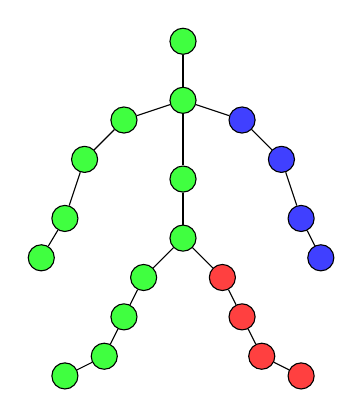
\begin{tikzpicture}
      \node[circle, draw, minimum size=0.1cm] (1) at (3.5,-1.25) [fill=green!75] {};
      \node[circle, draw, minimum size=0.1cm] (2) at (6.5, -1.25) [fill=red!75] {};
      \node[circle, draw, minimum size=0.1cm] (3) at (4,-1) [fill=green!75] {};
      \node[circle, draw, minimum size=0.1cm] (4) at (6, -1) [fill=red!75] {};
      \node[circle, draw, minimum size=0.1cm] (5) at (4.25,-0.5) [fill=green!75] {};
      \node[circle, draw, minimum size=0.1cm] (6) at (5.75,-0.5) [fill=red!75] {};
      \node[circle, draw, minimum size=0.1cm] (7) at (4.5,0) [fill=green!75] {};
      \node[circle, draw, minimum size=0.1cm] (8) at (5, 0.5) [fill=green!75] {};
      \node[circle, draw, minimum size=0.1cm] (9) at (5.5,0) [fill=red!75] {};
      \node[circle, draw, minimum size=0.1cm] (10) at (5,1.25) [fill=green!75] {};
      \node[circle, draw, minimum size=0.1cm] (11) at (3.2, 0.25) [fill=green!75] {};
      \node[circle, draw, minimum size=0.1cm] (12) at (6.75,0.25) [fill=blue!75] {};
      \node[circle, draw, minimum size=0.1cm] (13) at (3.5, 0.75) [fill=green!75] {};
      \node[circle, draw, minimum size=0.1cm] (14) at (6.5, 0.75) [fill=blue!75] {};
      \node[circle, draw, minimum size=0.1cm] (15) at (3.75,1.5) [fill=green!75] {};
      \node[circle, draw, minimum size=0.1cm] (16) at (6.25,1.5) [fill=blue!75] {};
      \node[circle, draw, minimum size=0.1cm] (17) at (4.25,2) [fill=green!75] {};
      \node[circle, draw, minimum size=0.1cm] (18) at (5,2.25) [fill=green!75] {};
      \node[circle, draw, minimum size=0.1cm] (19) at (5.75,2) [fill=blue!75] {};
      \node[circle, draw, minimum size=0.1cm] (20) at (5,3) [fill=green!75] {};  
      \foreach \source/\dest/\label/\xshiftval in {20/18//0, 18/17//0, 18/19//0, 17/15//0, 15/13//0, 13/11//0, 19/16//0, 16/14//0, 14/12//0, 18/10//0, 10/8//0, 8/7//0, 7/5//0, 5/3//0, 3/1//0, 8/9//0, 9/6//0, 6/4//0, 4/2//0}
        \path (\source) edge node[xshift=\xshiftval] {\label} (\dest);
    \end{tikzpicture}
    \caption{Graph $G$}
    \label{fig:graph_g}
  \end{subfigure}
  \hspace{0.01\linewidth}
  \begin{subfigure}{0.45\linewidth}
    \centering
    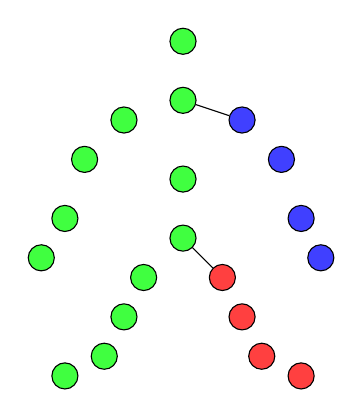
\begin{tikzpicture}
      \node[circle, draw, minimum size=0.1cm] (1) at (3.5,-1.25) [fill=green!75] {};
      \node[circle, draw, minimum size=0.1cm] (2) at (6.5, -1.25) [fill=red!75] {};
      \node[circle, draw, minimum size=0.1cm] (3) at (4,-1) [fill=green!75] {};
      \node[circle, draw, minimum size=0.1cm] (4) at (6, -1) [fill=red!75] {};
      \node[circle, draw, minimum size=0.1cm] (5) at (4.25,-0.5) [fill=green!75] {};
      \node[circle, draw, minimum size=0.1cm] (6) at (5.75,-0.5) [fill=red!75] {};
      \node[circle, draw, minimum size=0.1cm] (7) at (4.5,0) [fill=green!75] {};
      \node[circle, draw, minimum size=0.1cm] (8) at (5, 0.5) [fill=green!75] {};
      \node[circle, draw, minimum size=0.1cm] (9) at (5.5,0) [fill=red!75] {};
      \node[circle, draw, minimum size=0.1cm] (10) at (5,1.25) [fill=green!75] {};
      \node[circle, draw, minimum size=0.1cm] (11) at (3.2, 0.25) [fill=green!75] {};
      \node[circle, draw, minimum size=0.1cm] (12) at (6.75,0.25) [fill=blue!75] {};
      \node[circle, draw, minimum size=0.1cm] (13) at (3.5, 0.75) [fill=green!75] {};
      \node[circle, draw, minimum size=0.1cm] (14) at (6.5, 0.75) [fill=blue!75] {};
      \node[circle, draw, minimum size=0.1cm] (15) at (3.75,1.5) [fill=green!75] {};
      \node[circle, draw, minimum size=0.1cm] (16) at (6.25,1.5) [fill=blue!75] {};
      \node[circle, draw, minimum size=0.1cm] (17) at (4.25,2) [fill=green!75] {};
      \node[circle, draw, minimum size=0.1cm] (18) at (5,2.25) [fill=green!75] {};
      \node[circle, draw, minimum size=0.1cm] (19) at (5.75,2) [fill=blue!75] {};
      \node[circle, draw, minimum size=0.1cm] (20) at (5,3) [fill=green!75] {};  
      \foreach \source/\dest/\label/\xshiftval in {18/19//0, 8/9//0}
        \path (\source) edge node[xshift=\xshiftval] {\label} (\dest);
    \end{tikzpicture}
    \caption{Auxiliary graph $G^{aux}$}
    \label{fig:aux_graph}
  \end{subfigure}
\end{figure}


\subsection{Weighted Degree Centrality}
To identify the edge involved in the OoM, we use the WDC, as explained in Section \ref{subsec:weighted_degree}.
The calculation of the WDG is done on nodes, not on edges.
However, we will show how from a WDG calculated on nodes, we can derive the perceived movement origin on an edge.
For each frame, we keep track of the two nodes with the highest WDC.
Among the collected nodes, the two most frequent ones are selected across all frames.
At this stage, we will examine in the $G^{aux}$ to which edges belonging to $E^{aux}$ these two winning nodes are connected, and these two edges will be considered as the predicted OoM.
To achieve classification, finally, these two edges will be compared with the ground truth. 

\clearpage

\section{Visualization Framework}
This section aims to enhance the coherence of cluster visualization.
To achieve this goal, it is necessary to retrace the pipeline from Section \ref{sec:graph_method} to Section \ref{sec:spectral_clustering}.

\subsection{Temporal stabilization of clusters}
\label{subsec:clustering_stabilization}

After clustering, when visualizing their evolution over time, we observe a lack of consistency in subsequent assignments of colors. \\
As mentioned before, the order in which clusters are determined at each moment is random, and the selection order of clusters is represented by a color.
Therefore, from the initial random color assignment, we aim to transition to a color assignment where two clusters of the same color share as many nodes (joints) as possible over time.

This is because the random assignment of colors poses visualization issues for the graph.
It is possible that from one moment to the next, two clusters with many shared joints might have different colors, resulting in a visualization over time that appears as a continuous switching of colors. This could lead to a loss of continuity in the visual representation.
To stabilize clusters over time, ensuring that pairs of clusters colored from one moment to another share the highest number of common joints, we turn to the MaxWPM.

We have implemented two algorithms: a BF approach, where we compute the total weights of all possible permutations of color assignments and select the assignment with the maximum total weight, and the Hungarian Algorithm, a combinatorial optimization method that solves the assignment problem in polynomial time.

Since in our case the number of clusters is usually small, there are instances where the BF is more efficient.

\paragraph{Max Weight Perfect Matching}
Instead of the previously introduced nodes, we will have clusters, which are sets of nodes representing the joints of the skeleton, connected to each other by edges.\\  
Consider the clusters at time \textit{t} and the clusters at time \textit{t+1} as two distinct sets, so there will be no edges connecting clusters that belong to the same set.
Each cluster in one set must be connected by an edge to exactly one cluster in the other set, with the goal of maximizing the total weight of the edges.
The weight of an edge is equal to the number of nodes that the two clusters it is connecting have in common.\\
As previously mentioned, at this stage of the pipeline, we already have information about the joints belonging to various clusters and the colors of these clusters. However, we want to reassign colors to stabilize the visualization over time.
The previous clustering groups the joints into clusters and assigns them random colors, while in this phase of the pipeline, we optimize the color assignment.\\
We will start by analyzing the colors of the clusters at the initial frame and choose the best color assignment for the next frame.
Then will repeat this process iteratively until the last frame.\\

For example, we can consider a case that can we have frequently encountered in which the use of MaxWPM improved the visualization.
Let's suppose we have 20 nodes representing joints at time \textit{t} and 3 clusters labeled with different colors, as shown in Figure \ref{fig:clust_t}.
At time \textit{t+1}, there are the same 20 nodes as before but with 3 clusters changed but labeled using the same lexicographic order for the nodes (see Figure \ref{fig:clust_tplus1}). \\
Certainly, this clustering-based assignment cannot be regarded as the optimal assignment, as we still need to assess the \textit{3!} possible color assignments. \\
We know the colors of the clusters at time \textit{t}, and we want to assign colors to the clusters at time \textit{t+1}. \\
In Figure \ref{fig:clust_ass}, you can visually see all the possible color assignments, while in Table \ref{tab:table_clust}, all the values of common nodes for each color and the total weight of the matching are gathered.


\begin{figure}[H]
  \begin{subfigure}{\textwidth} % Adjust the width as needed
    \centering
    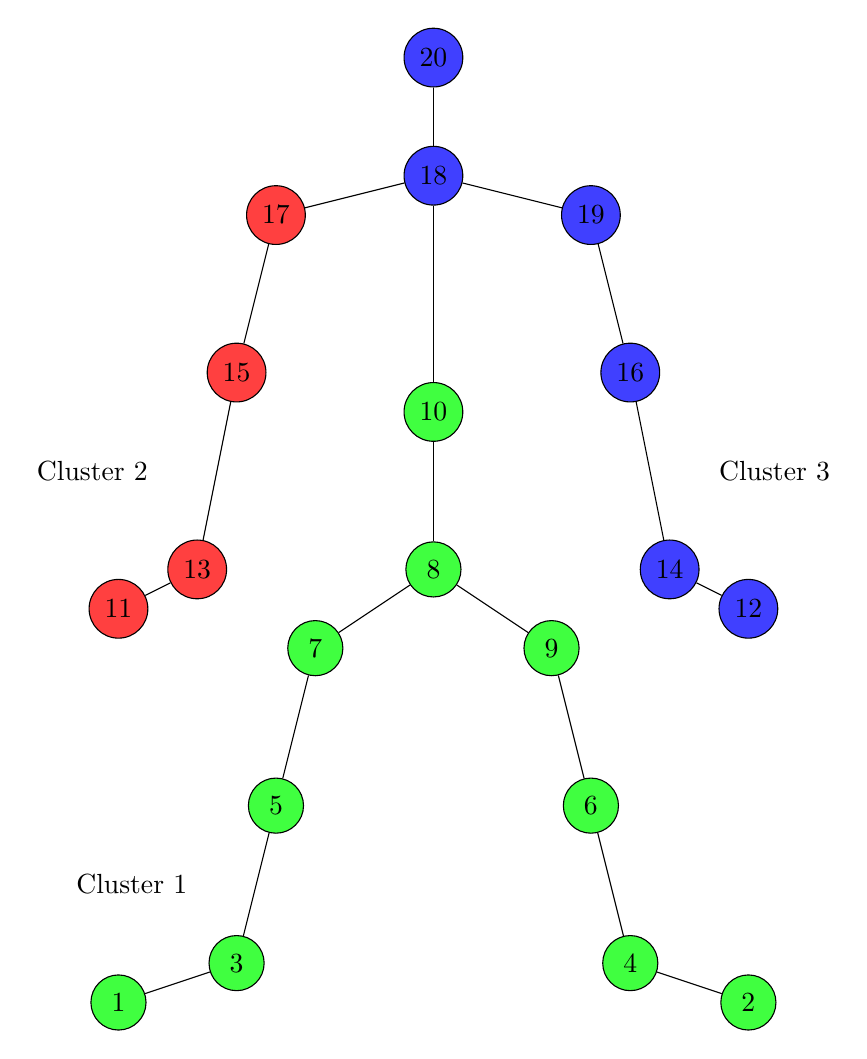
\begin{tikzpicture}
      \node[circle, draw, minimum size=0.7cm] (1) at (1,-9) [fill=green!75] {1};
      \node[circle, draw, minimum size=0.7cm] (2) at (9, -9) [fill=green!75] {2};
      \node[circle, draw, minimum size=0.7cm] (3) at (2.5,-8.5) [fill=green!75] {3};
      \node[circle, draw, minimum size=0.7cm] (4) at (7.5, -8.5) [fill=green!75] {4};
      \node[circle, draw, minimum size=0.7cm] (5) at (3,-6.5) [fill=green!75] {5};
      \node[circle, draw, minimum size=0.7cm] (6) at (7,-6.5) [fill=green!75] {6};
      \node[circle, draw, minimum size=0.7cm] (7) at (3.5,-4.5) [fill=green!75] {7};
      \node[circle, draw, minimum size=0.7cm] (8) at (5, -3.5) [fill=green!75] {8};
      \node[circle, draw, minimum size=0.7cm] (9) at (6.5,-4.5) [fill=green!75] {9};
      \node[circle, draw, minimum size=0.7cm] (10) at (5,-1.5) [fill=green!75] {10};
      \node[circle, draw, minimum size=0.7cm] (11) at (1,-4) [fill=red!75] {11};
      \node[circle, draw, minimum size=0.7cm] (12) at (9,-4) [fill=blue!75] {12};
      \node[circle, draw, minimum size=0.7cm] (13) at (2, -3.5) [fill=red!75] {13};
      \node[circle, draw, minimum size=0.7cm] (14) at (8, -3.5) [fill=blue!75] {14};
      \node[circle, draw, minimum size=0.7cm] (15) at (2.5,-1) [fill=red!75] {15};
      \node[circle, draw, minimum size=0.7cm] (16) at (7.5,-1) [fill=blue!75] {16};
      \node[circle, draw, minimum size=0.7cm] (17) at (3,1) [fill=red!75] {17};
      \node[circle, draw, minimum size=0.7cm] (18) at (5,1.5) [fill=blue!75] {18};
      \node[circle, draw, minimum size=0.7cm] (19) at (7,1) [fill=blue!75] {19};
      \node[circle, draw, minimum size=0.7cm] (20) at (5,3) [fill=blue!75] {20};
      \foreach \source/\dest/\label/\xshiftval in {20/18//0, 18/17//0, 18/19//0, 17/15//0, 15/13/Cluster 2/-45, 13/11//0, 19/16//0, 16/14/Cluster 3/45, 14/12//0, 18/10//0, 10/8//0, 8/7//0, 7/5//0, 5/3/Cluster 1/-45, 3/1//0, 8/9//0, 9/6//0, 6/4//0, 4/2//0}
        \path (\source) edge node[xshift=\xshiftval] {\label} (\dest);
    \end{tikzpicture}
    \caption{}
    \label{fig:clust_t}
  \end{subfigure}

  \vspace{1cm}

  \begin{subfigure}{\textwidth}
    \centering
    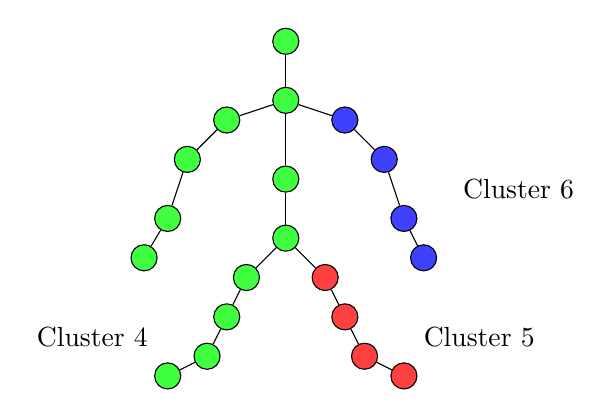
\begin{tikzpicture}
      \node[circle, draw, minimum size=0.3cm] (1) at (3.5,-1.25) [fill=green!75] {};
      \node[circle, draw, minimum size=0.3cm] (2) at (6.5, -1.25) [fill=red!75] {};
      \node[circle, draw, minimum size=0.3cm] (3) at (4,-1) [fill=green!75] {};
      \node[circle, draw, minimum size=0.3cm] (4) at (6, -1) [fill=red!75] {};
      \node[circle, draw, minimum size=0.3cm] (5) at (4.25,-0.5) [fill=green!75] {};
      \node[circle, draw, minimum size=0.3cm] (6) at (5.75,-0.5) [fill=red!75] {};
      \node[circle, draw, minimum size=0.3cm] (7) at (4.5,0) [fill=green!75] {};
      \node[circle, draw, minimum size=0.3cm] (8) at (5, 0.5) [fill=green!75] {};
      \node[circle, draw, minimum size=0.3cm] (9) at (5.5,0) [fill=red!75] {};
      \node[circle, draw, minimum size=0.3cm] (10) at (5,1.25) [fill=green!75] {};
      \node[circle, draw, minimum size=0.3cm] (11) at (3.2, 0.25) [fill=green!75] {};
      \node[circle, draw, minimum size=0.3cm] (12) at (6.75,0.25) [fill=blue!75] {};
      \node[circle, draw, minimum size=0.3cm] (13) at (3.5, 0.75) [fill=green!75] {};
      \node[circle, draw, minimum size=0.3cm] (14) at (6.5, 0.75) [fill=blue!75] {};
      \node[circle, draw, minimum size=0.3cm] (15) at (3.75,1.5) [fill=green!75] {};
      \node[circle, draw, minimum size=0.3cm] (16) at (6.25,1.5) [fill=blue!75] {};
      \node[circle, draw, minimum size=0.3cm] (17) at (4.25,2) [fill=green!75] {};
      \node[circle, draw, minimum size=0.3cm] (18) at (5,2.25) [fill=green!75] {};
      \node[circle, draw, minimum size=0.3cm] (19) at (5.75,2) [fill=blue!75] {};
      \node[circle, draw, minimum size=0.3cm] (20) at (5,3) [fill=green!75] {};  
      \foreach \source/\dest/\label/\xshiftval in {20/18//0, 18/17//0, 18/19//0, 17/15//0, 15/13//-45, 13/11//0, 19/16//0, 16/14/Cluster 6/45, 14/12//0, 18/10//0, 10/8//0, 8/7//0, 7/5//0, 5/3/Cluster 4/-45, 3/1//0, 8/9//0, 9/6//0, 6/4/Cluster 5/45, 4/2//0}
        \path (\source) edge node[xshift=\xshiftval] {\label} (\dest);
    \end{tikzpicture}
    \caption{}
    \label{fig:clust_tplus1}
  \end{subfigure}
  \caption{Color assignment at time \textit{t} (a) and \textit{t+1} (b)}
\end{figure}


\begin{figure}[H]
  \centering
  \begin{subfigure}{0.3\textwidth}
    \centering
    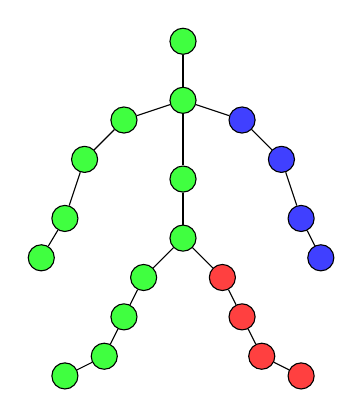
\begin{tikzpicture}[every node/.style={circle, draw, minimum size=0.1cm}]
      \node (1) at (3.5,-1.25) [fill=green!75] {};
      \node (2) at (6.5, -1.25) [fill=red!75] {};
      \node (3) at (4,-1) [fill=green!75] {};
      \node (4) at (6, -1) [fill=red!75] {};
      \node (5) at (4.25,-0.5) [fill=green!75] {};
      \node (6) at (5.75,-0.5) [fill=red!75] {};
      \node (7) at (4.5,0) [fill=green!75] {};
      \node (8) at (5, 0.5) [fill=green!75] {};
      \node (9) at (5.5,0) [fill=red!75] {};
      \node (10) at (5,1.25) [fill=green!75] {};
      \node (11) at (3.2, 0.25) [fill=green!75] {};
      \node (12) at (6.75,0.25) [fill=blue!75] {};
      \node (13) at (3.5, 0.75) [fill=green!75] {};
      \node (14) at (6.5, 0.75) [fill=blue!75] {};
      \node (15) at (3.75,1.5) [fill=green!75] {};
      \node (16) at (6.25,1.5) [fill=blue!75] {};
      \node (17) at (4.25,2) [fill=green!75] {};
      \node (18) at (5,2.25) [fill=green!75] {};
      \node (19) at (5.75,2) [fill=blue!75] {};
      \node (20) at (5,3) [fill=green!75] {};  
      \foreach \source/\dest in {20/18, 18/17, 18/19, 17/15, 15/13, 13/11, 19/16, 16/14, 14/12, 18/10, 10/8, 8/7, 7/5, 5/3, 3/1, 8/9, 9/6, 6/4, 4/2}
        \path (\source) edge (\dest);
    \end{tikzpicture}
    \caption{}
  \end{subfigure}
  \begin{subfigure}{0.3\textwidth}
    \centering
    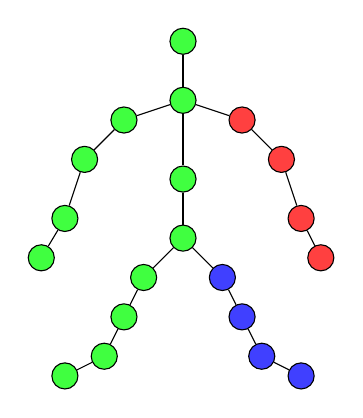
\begin{tikzpicture}[every node/.style={circle, draw, minimum size=0.1cm}]
      \node (1) at (3.5,-1.25) [fill=green!75] {};
      \node (2) at (6.5, -1.25) [fill=blue!75] {};
      \node (3) at (4,-1) [fill=green!75] {};
      \node (4) at (6, -1) [fill=blue!75] {};
      \node (5) at (4.25,-0.5) [fill=green!75] {};
      \node (6) at (5.75,-0.5) [fill=blue!75] {};
      \node (7) at (4.5,0) [fill=green!75] {};
      \node (8) at (5, 0.5) [fill=green!75] {};
      \node (9) at (5.5,0) [fill=blue!75] {};
      \node (10) at (5,1.25) [fill=green!75] {};
      \node (11) at (3.2, 0.25) [fill=green!75] {};
      \node (12) at (6.75,0.25) [fill=red!75] {};
      \node (13) at (3.5, 0.75) [fill=green!75] {};
      \node (14) at (6.5, 0.75) [fill=red!75] {};
      \node (15) at (3.75,1.5) [fill=green!75] {};
      \node (16) at (6.25,1.5) [fill=red!75] {};
      \node (17) at (4.25,2) [fill=green!75] {};
      \node (18) at (5,2.25) [fill=green!75] {};
      \node (19) at (5.75,2) [fill=red!75] {};
      \node (20) at (5,3) [fill=green!75] {};  
      \foreach \source/\dest in {20/18, 18/17, 18/19, 17/15, 15/13, 13/11, 19/16, 16/14, 14/12, 18/10, 10/8, 8/7, 7/5, 5/3, 3/1, 8/9, 9/6, 6/4, 4/2}
        \path (\source) edge (\dest);
    \end{tikzpicture}
      \caption{}
  \end{subfigure}
  \begin{subfigure}{0.3\textwidth}
    \centering
    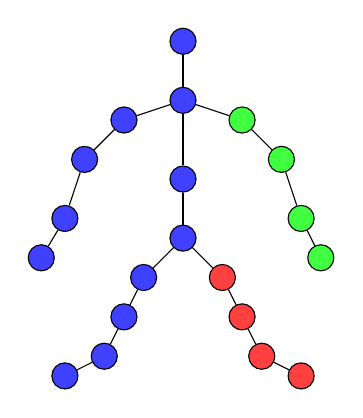
\begin{tikzpicture}[every node/.style={circle, draw, minimum size=0.1cm}]
      \node (1) at (3.5,-1.25) [fill=blue!75] {};
      \node (2) at (6.5, -1.25) [fill=red!75] {};
      \node (3) at (4,-1) [fill=blue!75] {};
      \node (4) at (6, -1) [fill=red!75] {};
      \node (5) at (4.25,-0.5) [fill=blue!75] {};
      \node (6) at (5.75,-0.5) [fill=red!75] {};
      \node (7) at (4.5,0) [fill=blue!75] {};
      \node (8) at (5, 0.5) [fill=blue!75] {};
      \node (9) at (5.5,0) [fill=red!75] {};
      \node (10) at (5,1.25) [fill=blue!75] {};
      \node (11) at (3.2, 0.25) [fill=blue!75] {};
      \node (12) at (6.75,0.25) [fill=green!75] {};
      \node (13) at (3.5, 0.75) [fill=blue!75] {};
      \node (14) at (6.5, 0.75) [fill=green!75] {};
      \node (15) at (3.75,1.5) [fill=blue!75] {};
      \node (16) at (6.25,1.5) [fill=green!75] {};
      \node (17) at (4.25,2) [fill=blue!75] {};
      \node (18) at (5,2.25) [fill=blue!75] {};
      \node (19) at (5.75,2) [fill=green!75] {};
      \node (20) at (5,3) [fill=blue!75] {};  
      \foreach \source/\dest in {20/18, 18/17, 18/19, 17/15, 15/13, 13/11, 19/16, 16/14, 14/12, 18/10, 10/8, 8/7, 7/5, 5/3, 3/1, 8/9, 9/6, 6/4, 4/2}
        \path (\source) edge (\dest);
    \end{tikzpicture}
      \caption{}
  \end{subfigure}
  
  \vspace{1cm} % Spazio vuoto tra le righe
  
  \begin{subfigure}{0.3\textwidth}
    \centering
    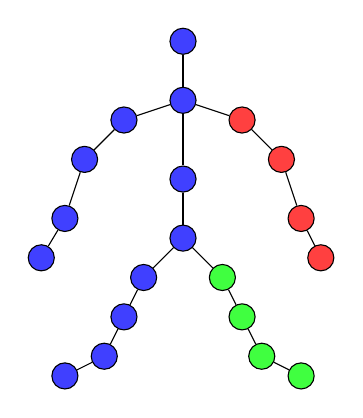
\begin{tikzpicture}[every node/.style={circle, draw, minimum size=0.1cm}]
      \node (1) at (3.5,-1.25) [fill=blue!75] {};
      \node (2) at (6.5, -1.25) [fill=green!75] {};
      \node (3) at (4,-1) [fill=blue!75] {};
      \node (4) at (6, -1) [fill=green!75] {};
      \node (5) at (4.25,-0.5) [fill=blue!75] {};
      \node (6) at (5.75,-0.5) [fill=green!75] {};
      \node (7) at (4.5,0) [fill=blue!75] {};
      \node (8) at (5, 0.5) [fill=blue!75] {};
      \node (9) at (5.5,0) [fill=green!75] {};
      \node (10) at (5,1.25) [fill=blue!75] {};
      \node (11) at (3.2, 0.25) [fill=blue!75] {};
      \node (12) at (6.75,0.25) [fill=red!75] {};
      \node (13) at (3.5, 0.75) [fill=blue!75] {};
      \node (14) at (6.5, 0.75) [fill=red!75] {};
      \node (15) at (3.75,1.5) [fill=blue!75] {};
      \node (16) at (6.25,1.5) [fill=red!75] {};
      \node (17) at (4.25,2) [fill=blue!75] {};
      \node (18) at (5,2.25) [fill=blue!75] {};
      \node (19) at (5.75,2) [fill=red!75] {};
      \node (20) at (5,3) [fill=blue!75] {};  
      \foreach \source/\dest in {20/18, 18/17, 18/19, 17/15, 15/13, 13/11, 19/16, 16/14, 14/12, 18/10, 10/8, 8/7, 7/5, 5/3, 3/1, 8/9, 9/6, 6/4, 4/2}
        \path (\source) edge (\dest);
    \end{tikzpicture}
      \caption{}
  \end{subfigure}
  \begin{subfigure}{0.3\textwidth}
    \centering
    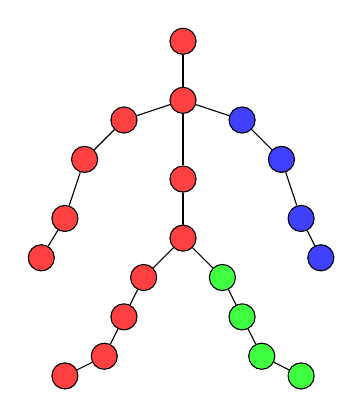
\begin{tikzpicture}[every node/.style={circle, draw, minimum size=0.1cm}]
      \node (1) at (3.5,-1.25) [fill=red!75] {};
      \node (2) at (6.5, -1.25) [fill=green!75] {};
      \node (3) at (4,-1) [fill=red!75] {};
      \node (4) at (6, -1) [fill=green!75] {};
      \node (5) at (4.25,-0.5) [fill=red!75] {};
      \node (6) at (5.75,-0.5) [fill=green!75] {};
      \node (7) at (4.5,0) [fill=red!75] {};
      \node (8) at (5, 0.5) [fill=red!75] {};
      \node (9) at (5.5,0) [fill=green!75] {};
      \node (10) at (5,1.25) [fill=red!75] {};
      \node (11) at (3.2, 0.25) [fill=red!75] {};
      \node (12) at (6.75,0.25) [fill=blue!75] {};
      \node (13) at (3.5, 0.75) [fill=red!75] {};
      \node (14) at (6.5, 0.75) [fill=blue!75] {};
      \node (15) at (3.75,1.5) [fill=red!75] {};
      \node (16) at (6.25,1.5) [fill=blue!75] {};
      \node (17) at (4.25,2) [fill=red!75] {};
      \node (18) at (5,2.25) [fill=red!75] {};
      \node (19) at (5.75,2) [fill=blue!75] {};
      \node (20) at (5,3) [fill=red!75] {};  
      \foreach \source/\dest in {20/18, 18/17, 18/19, 17/15, 15/13, 13/11, 19/16, 16/14, 14/12, 18/10, 10/8, 8/7, 7/5, 5/3, 3/1, 8/9, 9/6, 6/4, 4/2}
        \path (\source) edge (\dest);
    \end{tikzpicture}
      \caption{}
  \end{subfigure}
  \begin{subfigure}{0.3\textwidth}
    \centering
    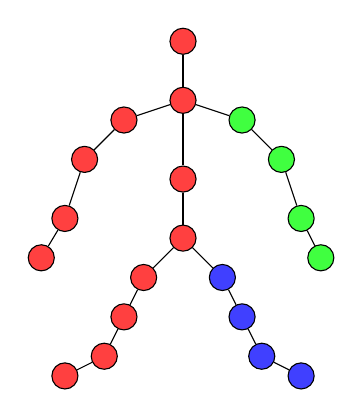
\begin{tikzpicture}[every node/.style={circle, draw, minimum size=0.1cm}]
      \node (1) at (3.5,-1.25) [fill=red!75] {};
      \node (2) at (6.5, -1.25) [fill=blue!75] {};
      \node (3) at (4,-1) [fill=red!75] {};
      \node (4) at (6, -1) [fill=blue!75] {};
      \node (5) at (4.25,-0.5) [fill=red!75] {};
      \node (6) at (5.75,-0.5) [fill=blue!75] {};
      \node (7) at (4.5,0) [fill=red!75] {};
      \node (8) at (5, 0.5) [fill=red!75] {};
      \node (9) at (5.5,0) [fill=blue!75] {};
      \node (10) at (5,1.25) [fill=red!75] {};
      \node (11) at (3.2, 0.25) [fill=red!75] {};
      \node (12) at (6.75,0.25) [fill=green!75] {};
      \node (13) at (3.5, 0.75) [fill=red!75] {};
      \node (14) at (6.5, 0.75) [fill=green!75] {};
      \node (15) at (3.75,1.5) [fill=red!75] {};
      \node (16) at (6.25,1.5) [fill=green!75] {};
      \node (17) at (4.25,2) [fill=red!75] {};
      \node (18) at (5,2.25) [fill=red!75] {};
      \node (19) at (5.75,2) [fill=green!75] {};
      \node (20) at (5,3) [fill=red!75] {};  
      \foreach \source/\dest in {20/18, 18/17, 18/19, 17/15, 15/13, 13/11, 19/16, 16/14, 14/12, 18/10, 10/8, 8/7, 7/5, 5/3, 3/1, 8/9, 9/6, 6/4, 4/2}
        \path (\source) edge (\dest);
    \end{tikzpicture}
      \caption{}
  \end{subfigure}

  \vspace{0.5cm} % Spazio vuoto tra le righe
  
  \caption{Possible color assignments at time \textit{t+1}}
  \label{fig:clust_ass}
\end{figure}



\begin{table}[H]
  \centering
  \begin{tabular}{||c||c||c||c||c||}
    \hline
   \textbf{Assignment} & \textbf{Red match} & \textbf{Blue match} & \textbf{Green match} & \textbf{Utility Value} \\
    \hline
    (a) & 0 & 4 & 6 & 10 \\
    \hline
    (b) & 0 & 0 & 6 & 6 \\
    \hline
    (c) & 0 & 2 & 0 & 2 \\
    \hline
    (d) & 0 & 2 & 4 & 6 \\
    \hline
    (e) & 4 & 4 & 4 & 12 \\
    \hline
    (f) & 4 & 0 & 0 & 4 \\
    \hline
  \end{tabular}
  
  \vspace{0.5cm} % Spazio vuoto tra le righe
  
  \caption{Matching weights for the 6 assignments}
  \label{tab:table_clust}
\end{table}
\clearpage 
From Table \ref{tab:table_clust}, it can be observed that assignment (e) has the highest utility value.
Additionally, even visually, it can be noticed that it is the most consistent assignment compared to the one at time \textit{t}.
\\

From the perspective of Bipartite Matching, we can consider the clusters from Figure \ref{fig:clust_t} in the first partition, while in the second partition, we can consider the clusters from Figure \ref{fig:clust_tplus1}.
As mentioned earlier, the weight of an edge is equivalent to the number of nodes that the two clusters being connected by that edge have in common. \\
The following figure shows the matching with the utility value for every possible assignment and the colored ones for the optimal one.



\begin{figure}[H]
  \centering
  \begin{minipage}{0.45\textwidth}
    \centering
    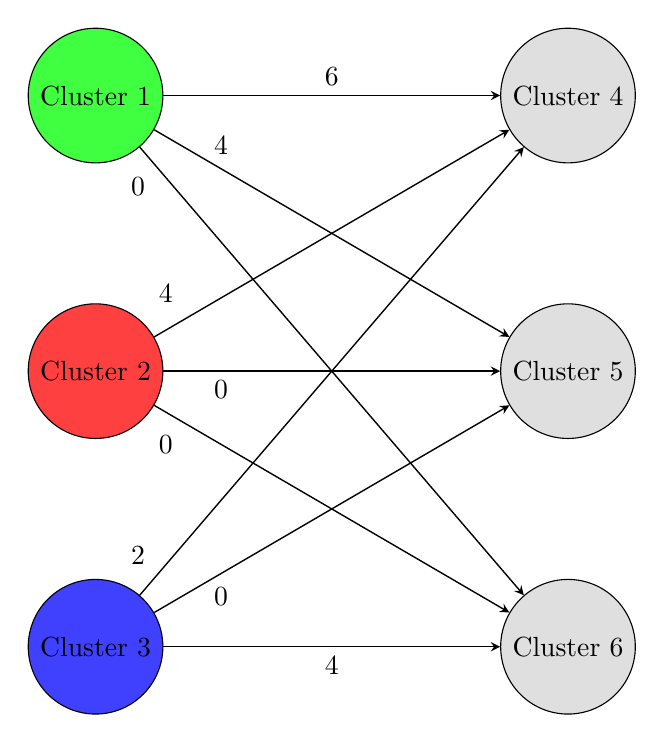
\begin{tikzpicture}
      \node[circle, draw, minimum size=1cm, fill=green!75] (1) at (2,-6.5) {Cluster 1};
      \node[circle, draw, minimum size=1cm, fill=red!75] (2) at (2, -10) {Cluster 2};
      \node[circle, draw, minimum size=1cm, fill=blue!75] (3) at (2,-13.5) {Cluster 3};
      \node[circle, draw, minimum size=1cm, fill=gray!25] (4) at (8, -6.5) {Cluster 4};
      \node[circle, draw, minimum size=1cm, fill=gray!25] (5) at (8,-10) {Cluster 5};
      \node[circle, draw, minimum size=1cm, fill=gray!25] (6) at (8,-13.5) {Cluster 6};
      
      \foreach \source/\dest/\label/\position/\yshiftval/\xshiftval/\edgecolor in {
        1/4/6/above/0/0/black, 1/5/4/above/25/-40/black, 1/6/0/above/60/-70/black,
        2/4/4/below/-15/-60/black, 2/5/0/below/0/-40/black, 2/6/0/below/30/-60/black,
        3/4/2/below/-60/-70/black, 3/5/0/below/-25/-40/black, 3/6/4/below/0/0/black}
        \path (\source) edge[\edgecolor, ->,>=stealth, line width=0.5pt] node[\position, yshift=\yshiftval, xshift=\xshiftval, black] {\label} (\dest);
    \end{tikzpicture}
  \end{minipage}
  \hfill
  \begin{minipage}{0.45\textwidth}
    \centering
    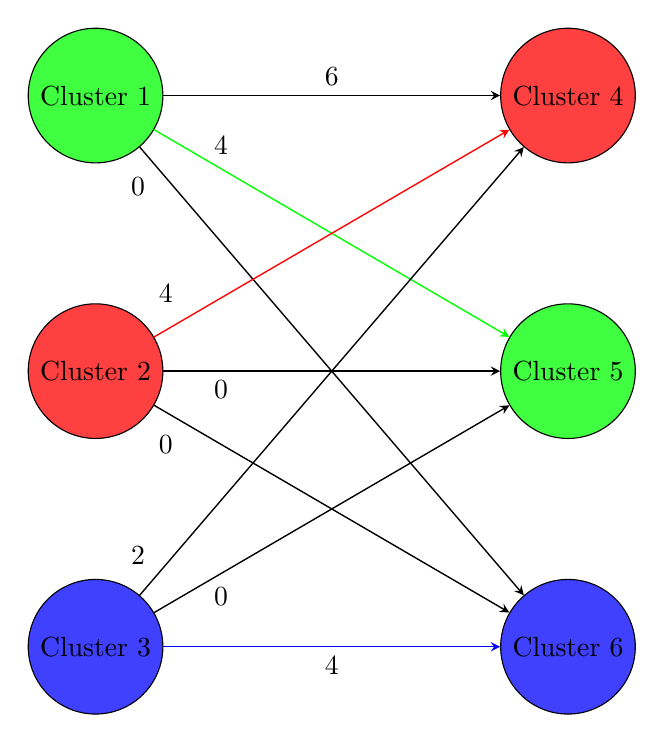
\begin{tikzpicture}
      \node[circle, draw, minimum size=1cm, fill=green!75] (1) at (2,-6.5) {Cluster 1};
      \node[circle, draw, minimum size=1cm, fill=red!75] (2) at (2, -10) {Cluster 2};
      \node[circle, draw, minimum size=1cm, fill=blue!75] (3) at (2,-13.5) {Cluster 3};
      \node[circle, draw, minimum size=1cm, fill=red!75] (4) at (8, -6.5) {Cluster 4};
      \node[circle, draw, minimum size=1cm, fill=green!75] (5) at (8,-10) {Cluster 5};
      \node[circle, draw, minimum size=1cm, fill=blue!75] (6) at (8,-13.5) {Cluster 6};
      
      \foreach \source/\dest/\label/\position/\yshiftval/\xshiftval/\edgecolor in {
        1/4/6/above/0/0/black, 1/5/4/above/25/-40/green, 1/6/0/above/60/-70/black,
        2/4/4/below/-15/-60/red, 2/5/0/below/0/-40/black, 2/6/0/below/30/-60/black,
        3/4/2/below/-60/-70/black, 3/5/0/below/-25/-40/black, 3/6/4/below/0/0/blue}
        \path (\source) edge[\edgecolor, ->,>=stealth, line width=0.5pt] node[\position, yshift=\yshiftval, xshift=\xshiftval, black] {\label} (\dest);
    \end{tikzpicture}
  \end{minipage}
  \caption{Bipartite Matching from instant \textit{t} to instant \textit{t+1}}
  \label{fig:clust_match}
\end{figure}
We explored two algorithmns for computing the MaxWPM.
\clearpage

\paragraph{Hungarian Matching}
One approach consists in applying the Hungarian Algorithm which is a combinatorial optimization algorithm that also solves the assignment problem.\\
Now let's see the previous example solved with this algorithm in the Table \ref{tab:hung_alg_appl}:
The initial step (a) involves working with a table describing the utility values associated with each assignment. Each cell in this table represents the cost or utility of assigning a task to a resource.

In (b) we inverted each element in the table to obtain the cost value associated with each assignment. This step transforms the utility table into a cost table, turning the problem into a minimization one.

For each row in the cost table, subtract the smallest value in that row from all the elements (c).

Similarly, for each column in the table, subtract the smallest value in that column from all the elements (d).

Draw the minimum number of lines required to cover rows and columns that have zero entries (e). Since the number of lines equals the number of rows, we can already reach an optimal solution.

Starting from the top-left corner, select a zero that doesn't cover any other zeros (f). This selection initiates the assignment process.

Continue by selecting cells that cover the minimum number of zeros for each row and are not in columns that have already been covered (g).

Proceed by selecting the remaining cell that hasn't been covered by any column (h). We reached the end of the assignment process.

Finally, revert back to the original cost matrix (i).

\begin{table}[H]
  \centering
  \begin{minipage}{0.3\textwidth}
    \centering
    \begin{tabular}{|>{\centering\arraybackslash}m{0.6cm}|>{\centering\arraybackslash}m{0.6cm}|>{\centering\arraybackslash}m{0.6cm}|}
      \hline
      6 & 4 & 0 \\
      \hline
      4 & 0 & 0 \\
      \hline
      2 & 0 & 4 \\
      \hline
    \end{tabular}
    \caption*{(a)}
  \end{minipage}
  \hfill
  \begin{minipage}{0.3\textwidth}
    \centering
    \begin{tabular}{|>{\centering\arraybackslash}m{0.6cm}|>{\centering\arraybackslash}m{0.6cm}|>{\centering\arraybackslash}m{0.6cm}|}
      \hline
      -6 & -4 & 0 \\
      \hline
      -4 & 0 & 0 \\
      \hline
      -2 & 0 & -4 \\
      \hline
    \end{tabular}
    \caption*{(b)}
  \end{minipage}
  \hfill
  \begin{minipage}{0.3\textwidth}
    \centering
    \begin{tabular}{|>{\centering\arraybackslash}m{0.6cm}|>{\centering\arraybackslash}m{0.6cm}|>{\centering\arraybackslash}m{0.6cm}|}
      \hline
      0 & 2 & 6 \\
      \hline
      0 & 4 & 4 \\
      \hline
      2 & 4 & 0 \\
      \hline
    \end{tabular}
    \caption*{(c)}
  \end{minipage}

  \vspace{5pt}

  \begin{minipage}{0.3\textwidth}
    \centering
    \begin{tabular}{|>{\centering\arraybackslash}m{0.6cm}|>{\centering\arraybackslash}m{0.6cm}|>{\centering\arraybackslash}m{0.6cm}|}
      \hline
      0 & 0 & 6 \\
      \hline
      0 & 2 & 4 \\
      \hline
      2 & 2 & 0 \\
      \hline
    \end{tabular}
    \caption*{(d)}
  \end{minipage}
  \hfill
  \begin{minipage}{0.3\textwidth}
    \centering
    \begin{tabular}{|>{\centering\arraybackslash}m{0.6cm}|>{\centering\arraybackslash}m{0.6cm}|>{\centering\arraybackslash}m{0.6cm}|}
      \hline
      \cellcolor{gray!25} 0 & \cellcolor{gray!25} 0 & \cellcolor{gray!25} 6 \\
      \hline
      \cellcolor{gray!25} 0 & \cellcolor{gray!25} 2 & \cellcolor{gray!25} 4 \\
      \hline
      2 & 2 & \cellcolor{gray!25} 0 \\
      \hline
    \end{tabular}
    \caption*{(e)}
  \end{minipage}
  \hfill
  \begin{minipage}{0.3\textwidth}
    \centering
    \begin{tabular}{|>{\centering\arraybackslash}m{0.6cm}|>{\centering\arraybackslash}m{0.6cm}|>{\centering\arraybackslash}m{0.6cm}|}
      \hline
      \cellcolor{gray!25} 0 & \cellcolor{gray!25} 0 & \cellcolor{gray!25} 6 \\
      \hline
      \cellcolor{green!75} 0 & \cellcolor{gray!25} 2 & \cellcolor{gray!25} 4 \\
      \hline
      2 & 2 & \cellcolor{gray!25} 0 \\
      \hline
    \end{tabular}
    \caption*{(f)}
  \end{minipage}

  \vspace{5pt}

  \begin{minipage}{0.3\textwidth}
    \centering
    \begin{tabular}{|>{\centering\arraybackslash}m{0.6cm}|>{\centering\arraybackslash}m{0.6cm}|>{\centering\arraybackslash}m{0.6cm}|}
      \hline
      \cellcolor{gray!25} 0 & \cellcolor{gray!25} 0 & \cellcolor{gray!25} 6 \\
      \hline
      \cellcolor{green!75} 0 & \cellcolor{gray!25} 2 & \cellcolor{gray!25} 4 \\
      \hline
      2 & 2 & \cellcolor{green!75} 0 \\
      \hline
    \end{tabular}
    \caption*{(g)}
  \end{minipage}
  \hfill
  \begin{minipage}{0.3\textwidth}
    \centering
    \begin{tabular}{|>{\centering\arraybackslash}m{0.6cm}|>{\centering\arraybackslash}m{0.6cm}|>{\centering\arraybackslash}m{0.6cm}|}
      \hline
      0 & \cellcolor{green!75} 0 & 6 \\
      \hline
      \cellcolor{green!75} 0 & 2 & 4 \\
      \hline
      2 & 2 & \cellcolor{green!75} 0 \\
      \hline
    \end{tabular}
    \caption*{(h)}
  \end{minipage}
  \hfill
  \begin{minipage}{0.3\textwidth}
    \centering
    \begin{tabular}{|>{\centering\arraybackslash}m{0.6cm}|>{\centering\arraybackslash}m{0.6cm}|>{\centering\arraybackslash}m{0.6cm}|}
      \hline
      6 & \cellcolor{green!75} 4 & 0 \\
      \hline
      \cellcolor{green!75} 4 & 0 & 0 \\
      \hline
      2 & 0 & \cellcolor{green!75} 4 \\
      \hline
    \end{tabular}
    \caption*{(i)}
  \end{minipage}
  \caption{Application of the Hungarian Algorithm to clusters stabilization}
  \label{tab:hung_alg_appl}
\end{table}

\paragraph{Brute Force} Another approach consists in a brute force method for choosing an option based on the minimum sum of utility values of a graph involves exhaustively evaluating every possible combination of options to find the one with the highest total weight. 
This method consists of enumerating all possible subsets or combinations of options within the graph, computing theier sum of weights, ranking results and choosing the best one.
It can be also used to validate the first one.
The Table \ref{tab:bf_alg} is a clear example of this approach. \\   

\begin{table}[H]
  \centering
  \begin{minipage}{0.3\textwidth}
    \centering
    \begin{tabular}{|>{\centering\arraybackslash}m{0.6cm}|>{\centering\arraybackslash}m{0.6cm}|>{\centering\arraybackslash}m{0.6cm}|}
      \hline
      \cellcolor{green!75}-6 & -4 & 0 \\
      \hline
      -4 & \cellcolor{green!75}0 & 0 \\
      \hline
      -2 & 0 & \cellcolor{green!75}-4 \\
      \hline
    \end{tabular}
    \caption*{(a)}
  \end{minipage}
  \hfill
  \begin{minipage}{0.3\textwidth}
    \centering
    \begin{tabular}{|>{\centering\arraybackslash}m{0.6cm}|>{\centering\arraybackslash}m{0.6cm}|>{\centering\arraybackslash}m{0.6cm}|}
      \hline
      \cellcolor{green!75}-6 & -4 & 0 \\
      \hline
      -4 & 0 & \cellcolor{green!75}0 \\
      \hline
      -2 & \cellcolor{green!75}0 & -4 \\
      \hline
    \end{tabular}
    \caption*{(b)}
  \end{minipage}
  \hfill
  \begin{minipage}{0.3\textwidth}
    \centering
    \begin{tabular}{|>{\centering\arraybackslash}m{0.6cm}|>{\centering\arraybackslash}m{0.6cm}|>{\centering\arraybackslash}m{0.6cm}|}
      \hline
      -6 & -4 & \cellcolor{green!75}0 \\
      \hline
      -4 & \cellcolor{green!75}0 & 0 \\
      \hline
      \cellcolor{green!75}-2 & 0 & -4 \\
      \hline
    \end{tabular}
    \caption*{(c)}
  \end{minipage}

  \vspace{10pt}

  \begin{minipage}{0.3\textwidth}
    \centering
    \begin{tabular}{|>{\centering\arraybackslash}m{0.6cm}|>{\centering\arraybackslash}m{0.6cm}|>{\centering\arraybackslash}m{0.6cm}|}
      \hline
      -6 & \cellcolor{green!75}-4 & 0 \\
      \hline
      -4 & 0 & \cellcolor{green!75}0 \\
      \hline
      \cellcolor{green!75}-2 & 0 & -4 \\
      \hline
    \end{tabular}
    \caption*{(d)}
  \end{minipage}
  \hfill
  \begin{minipage}{0.3\textwidth}
    \centering  
    \begin{tabular}{|>{\centering\arraybackslash}m{0.6cm}|>{\centering\arraybackslash}m{0.6cm}|>{\centering\arraybackslash}m{0.6cm}|}
      \hline
      -6 & \cellcolor{green!75}-4 & 0 \\
      \hline
      \cellcolor{green!75}-4 & 0 & 0 \\
      \hline
      -2 & 0 & \cellcolor{green!75}-4 \\
      \hline
    \end{tabular}
    \caption*{(e)}
  \end{minipage}
  \hfill
  \begin{minipage}{0.3\textwidth}
    \centering
    \begin{tabular}{|>{\centering\arraybackslash}m{0.6cm}|>{\centering\arraybackslash}m{0.6cm}|>{\centering\arraybackslash}m{0.6cm}|}
      \hline
      -6 & -4 & \cellcolor{green!75}0 \\
      \hline
      \cellcolor{green!75}-4 & 0 & 0 \\
      \hline
      -2 & \cellcolor{green!75}0 & -4 \\
      \hline
    \end{tabular}
    \caption*{(f)}
  \end{minipage}
  \caption{Real application of the BF Algorithm}
  \label{tab:bf_alg}
\end{table}


BF approach guarantees finding the best option, it can be computationally expensive, especially for large graphs.
As we can see, here we have the computation of all the \textit{n!} permutations and the minimum one is (e).

\subsection{Clustering Transition Smoothing}
\label{subsec:clusters_smoothing}

After achieving cluster stabilization at the interframe level, a persistent issue remains. 
Despite the smoothness of actual movements, the transition of a cluster from a part of the body is still too fast.
This is due to the fact that is a greedy approach and is not considering the temporal progression of clusters.
To address this issue a delay and smoothing procedure has been used.
It consists in computing the difference between the sets representing clusters at time t+1 and clusters at time t.
Apply the weighted degree centrality to the nodes within each cluster in the resulting set, and select the maximum value.
For each cluster, update the label of the node with the highest weighted degree centrality.
This algorithm is applied only every $k = \frac{1}{4}framerate$ time instant, effectively updating the clusters, in the other time instants these are not updated.

By parameterizing $k$ this process appropriately to ensure that clusters do not undergo excessive changes during this time interval, an oscillating effect is achieved. 
This effect propagates the cluster across the connected nodes that belong to it, thereby making any potential origin of the movement more conspicuous.

\clearpage
\section{Machine Learning Framework}
\label{sec:ml_method}
In this section, we describe the process of extracting and engineering features from the raw data, the process to refine the model in order to obtain highly accurate model, and the different formulations of binary questions posed to it.

\subsection{Features engineering}
The initial dataset we started from, as described in Section \ref{sec:annotations}, consists of 60 time series of the 20 joints trajectories.
In order to avoid noise or presence of more origin of movements, we trimmed the videos finely, resulting in clips of variable lengths ($\mu = 1.96s , \sigma^{2} = 1.49s$).

\paragraph{Frames sampling} To address the variable length of segments within the dataset, in instances where we aim to attain a uniform number of frames than the actual length of the segments, 
we have utilized the \textit{uniform spacing sampling} technique to address the variability in segment lengths within the dataset.
This method entails selecting frames from a list or sequence at regular, even intervals, by fixing a number of frames that we wanted, in our case 200, and then keeping only those frames equally spaced between eachother.

Conversely, when dealing with segments that are shorter than the required number of frames, a different technique is implemented.
In such cases, for each frame, a variable and uniform number of interpolation frames are inserted to reach the desired frame count. 
This approach compensates for the shorter segment length by adding approximately the same amount of interpolated frames across the whole segment, maintaining the consistency required for the following statistical analysis.


\paragraph{Dataset Normalization}
From the timeseries produced by the sampling process we calculate the $x$, $y$, and $z$ coordinates of the skeleton's barycenter for each time step. \\
We define the barycenter as the point where all the mass of an object or a system of objects is concentrated. \\
In this context, each joint is considered to have unit mass, meaning that all joints contribute equally to the barycenter. \\
If we represent $n$ as the number of 20 joints, the coordinates of the barycenter are obtained by taking the average of the coordinates of these 20 joints, as we can see in the formula:

\begin{equation}
    Barycenter (x, y, z) = \left(\frac{1}{n} \sum_{i=1}^{n} x_i, \frac{1}{n} \sum_{i=1}^{n} y_i, \frac{1}{n} \sum_{i=1}^{n} z_i\right)
    \label{formula:baricentro}
\end{equation}
    
where $x_i$, $y_i$, and $z_i$ represent the $x$, $y$, and $z$ coordinates of the $i$-th joint, respectively.

Subsequently, we calculate the distance between each joint and the barycenter, at each time step, using the Euclidean distance in Formula \ref{formula:distance}. \\
These distances from the barycenter will be normalized for each joint, in order to obtain a time series whose values space between 0 and 1.

\begin{equation}
    x_{norm} = \frac{{x - min(x)}}{{max(x) - min(x)}}
    \label{formula:normalization}
\end{equation}
    
The choice to calculate the distances between joints and the barycenter for each sample plays a crucial role in ensuring the robustness of our ML approach to variations in scale.
In scenarios where dancers or subjects may have different heights or body proportions, relying solely on absolute joint coordinates could introduce bias into the model.
However, by computing these distances and further normalizing them within the range of 0 to 1, we effectively eliminate the influence of scale variations.

\paragraph{Features extraction}
This process involves transforming raw data into a more suitable format for analysis and model building.
Here are all the functions calculated for every sample of the dataset (note that \textit{n} is the number of frames of the sample). \\

\textbf{Mean} is the expected value of the distribution:
        \begin{equation}
            \mu = \frac{1}{n} \sum_{i=1}^{n} x_i
        \end{equation}
\textbf{Variance} is the second momentum of the distribution (or the squared deviation of the expected value from the mean):
        \begin{align}
          \sigma^2 &= \mu_2 &
          \mu_k &= \frac{1}{n} \sum_{i=1}^{n} (x_i - \mu)^k 
        \end{align}
\textbf{Kurtosis} is the fourth standardized moment:
        \begin{equation}
            Kurt[X] = \frac{\mu_4}{\sigma^4} - 3
        \end{equation}
\textbf{Skewness} is the third standardized moment:
        \begin{equation}
            \gamma_1 = \frac{\mu_3}{\sigma^3}
        \end{equation}
\textbf{Mean Standard Error}:
        \begin{equation}
            \sigma_{\bar{x}} = \sqrt{\frac{\sigma^2}{n}}
        \end{equation}
\textbf{Correlation} between two joints (\textit{x},\textit{y}):
        \begin{equation}
            \rho_{X,Y} = \frac{\sum_{i=1}^n (x_i - \mu_{X})(y_i - \mu_{Y})}{\sigma_{X}\cdot\sigma_{Y}}
        \end{equation}
\textbf{Mean Absolute Deviation}:
        \begin{equation}
            mad(\bar{x}) = \frac{1}{n} \sum_{i=1}^{n} |x_i - \mu|
        \end{equation}
\textbf{Average Sum of Squares}:
        \begin{equation}
            energy(\bar{x}) = \sqrt{\sum_{i=1}^{n} x_i^2}
        \end{equation}
\textbf{Interquantile Range} measures statistical dispersion in the range between the 25th (Q1) and the 75th percentile (Q3) of the data distribution ($ iqr = Q3 - Q1 $):
        \begin{equation}
            iqr(\bar{x}) =  
                \begin{cases} 
                \bar{x}_{\frac{3}{4}(n+1)} - \bar{x}_{(\frac{n+1}{4})} & \text{if n is odd} \\
                \frac{(\bar{x}_{(\frac{3}{4}n)} + \bar{x}_{(\frac{3}{4}n+1)}) - (\bar{x}_{(\frac{n}{4})} + \bar{x}_{(\frac{n}{4}+1)})}{2} & \text{otherwise}
                \end{cases}
        \end{equation}
        \begin{figure}[H]
            \centering
            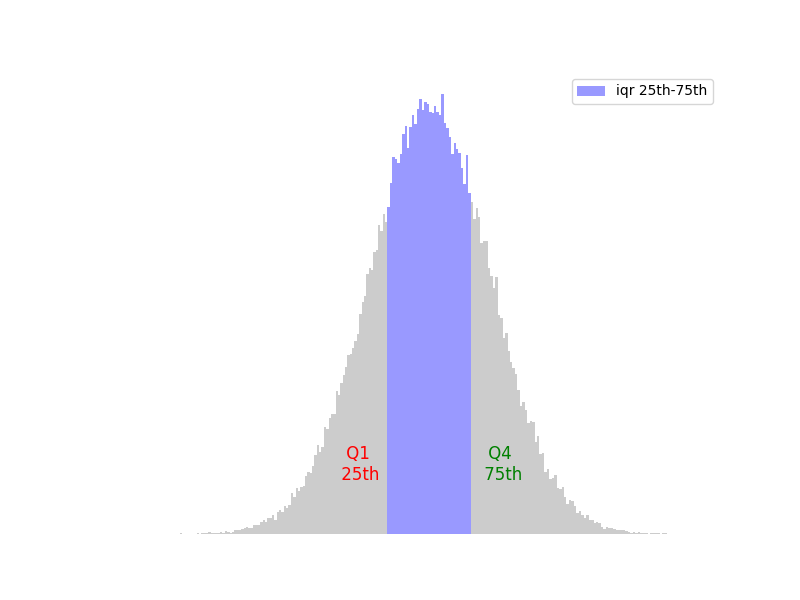
\includegraphics[width=0.85\textwidth]{iqr.png}
            \caption{Interquantile range of a normal distribution}
            \label{fig:iqr}
        \end{figure}
\textbf{Fundamental Frequency Signal} from the Discrete Fourier Transform (DFT):
    \begin{equation}
        firstFreq(\bar{x}) = \angle DFT(\bar{x})[1]
    \end{equation}
\textbf{Real part's Average of Frequency Signal}:
    \begin{equation}
        meanFreq(\bar{x}) = \sum_{i=1}^{n} Re(DFT(x_i))
    \end{equation}
\textbf{Real part's Max of Frequency Signal}:
    \begin{equation}
        maxFreq(\bar{x}) = Max(Re(DFT(x)))
    \end{equation}
\textbf{Index of the Max of the Real part of Frequency Signal}:
    \begin{equation}
        maxFreq(\bar{x}) = Argmax(Re(DFT(x)))
    \end{equation}

The last four values correspond to the minimum value and its index, skewness, and kurtosis of the Fourier transform.
To choose the features to extract, we referred to \cite{oneto:2020} and \cite{sama:2010}.
In Table \ref{tab:ml_features} we can see all the features and their relative function.

\begin{table}[H]
    \centering
    \begin{tabular}{||c||c||}
        \hline
        \textbf{Function} & \textbf{Description} \\
        \hline
        mean & Mean \\
        var & Variance \\
        kurt & Kurtosis \\
        skew & Skewness \\
        corr & Correlation Coefficient \\
        mad & Mean Absolute Deviation \\
        sem & Mean Standard Error \\
        energy & Average Sum of Squares \\
        iqr & Interquantile Range \\
        min & Smallest Value in Array \\
        max & Largest Value in Array \\
        firstFreq & Fundamental Frequency Signal \\
        meanFreq & Real part's Average of Frequency Signal \\
        maxFreq & Real part's Max of Frequency Signal \\
        maxFreqIndx & Index of the Max of the Real part of Frequency Signal \\ 
        minFreq & Real part's Min of Frequency Signal \\
        minFreqIndx & Index of the Min of the Real part of Frequency Signal \\ 
        skewFreq & Frequency Signal Skewness \\
        kurtFreq & Frequency Signal Kurtosis \\
        \hline
    \end{tabular}
    \caption{List of measures for computing feature vectors}
\label{tab:ml_features}
\end{table}

Here is the operative Python code for the extraction of the features from the raw data after the normalization.
\clearpage 
\lstsetlarge
\lstinputlisting[firstline=1, lastline=30]{code/ml.py}

\subsection{Classification}
The initial approach involves a simple binary classification of the origin of the movement in a specific edge or not.
If the results had been satisfactory, we would then have opted to evaluate progressively more complex models, eventually leading to the multiclass classification.
We started by addressing the issue of imbalanced data in classification.
The choice of LOOCV was motivated by the presence of a very small dataset, allowing us to compute the maximum number of training cycles to have a virtually unbiased model.

To mitigate this imbalance, a resampling technique known as B-SMOTE is employed (\textit{BS1}). 
This technique equalizes the number of training samples for the minority class with that of the majority class at each iteration.
B-SMOTE generates additional samples for the minority class to balance the number of samples of the majority class.
For instance, if there are 50 samples of one class and 9 of the other during a training step, B-SMOTE will artificially create 41 samples for the second class. \\
The operational concept is detailed in Section \ref{subsec:borderline}.

Following the resampling of the training data, a RF classifier (\textit{RF1}) is trained on this newly balanced dataset.
To further optimize the classifier's performance, a feature selection process is employed with the goal of identifying the most influential features that contribute to accurate classification.
The most important features are determined through the training of \textit{RF1} on the resampled data. 
These features are selected based on the amount of information that they provide in the classification task weighting Gini importance of the feature across all the trees. \\
Subsequently, a new RF classifier (\textit{RF2}) is trained using only the 50 most important features of the previous model, with the \textit{max\_features} hyperparameter tuned to choose among all the available features in each split.
To evaluate the performance of the classifier, a test set is chosen using LOOCV, as detailed in Section \ref{subsec:cross_validation}. 

\begin{table}[H]
    \centering
    \begin{tabular}{||c||c||c||}
        \hline
        \textbf{Model} & \textbf{Hyperparameter} & \textbf{Value} \\
        \hline
        \textit{BS1} & \textit{k}-\textit{neighbors} & 0.4 $\cdot$ count(Less Frequent Class)  \\
        & \textit{m}-\textit{neighbors} & 0.4 $\cdot$ count(Most Frequent Class)  \\
        \hline
        \textit{RF1} & \textit{n}\_\textit{estimators} & 500  \\
        & \textit{max}\_\textit{features} & Default  \\
        \hline
        \textit{RF2} & \textit{n}\_\textit{estimators} & 200  \\
        & \textit{max}\_\textit{features} & All  \\
        \hline
    \end{tabular}
    \caption{Hyperparameters tuned for our application}
    \label{tab:ml_param}
\end{table}

Below is the code used to train and test the RF with the aforementioned parameters.
\clearpage
\lstsetnormal
\lstinputlisting[firstline=33, lastline=77]{code/ml.py}

In our ML model, we posed three different questions regarding the OoM. 
Since our dataset is inherently a multi-class dataset, we performed binary classification by reclassifying the dataset based on our necessities.
These binary questions are posed either to edges or to specific parts of the skeleton, which are themselves composed of edges. \\
In Figures \ref{tab:ml_division_5_body_parts} and \ref{tab:ml_division_top_bottom}, you can see the edges composing different segments of the skeleton. \\
Note that not every edge of the reduced marker set (\ref{tab:labels_joints}) is included because some edges have not been the ground truth for any sample in our dataset.
For ML we have in total 15 classes, that is 15 edges.
After each reclassification the same pipeline of training and testing is used.

\begin{table}[H]
    \centering
    \renewcommand{\arraystretch}{1.2}
    \begin{subtable}{\textwidth}
        \centering
        \begin{tabular}{||c||c||}
            \hline
            \textbf{Body Part} & \textbf{Edges} \\
            \hline
            Head & shoulder\_center - head \\
            \hline
            Right Arm & right\_hand - right\_wrist \\
            & right\_wrist - right\_elbow \\
            & right\_elbow - right\_shoulder \\
            & right\_shoulder - shoulder\_center \\
            \hline
            Left Arm & left\_hand - left\_wrist \\
            & left\_elbow - left\_shoulder \\
            & left\_shoulder - shoulder\_center \\
            \hline
            Right Leg & right\_foot - right\_ankle \\
            & right\_ankle - right\_knee \\
            & right\_knee - right\_hip \\
            & right\_hip - hip\_center \\
            \hline
            Left Leg & left\_foot - left\_ankle \\
            & left\_knee - left\_hip \\
            & left\_hip - hip\_center \\
            \hline
        \end{tabular}
        \caption{}
        \label{tab:ml_division_5_body_parts}
    \end{subtable}

    \vspace{10pt} % Add vertical space between subtables

    \begin{subtable}{\textwidth}
        \centering
        \begin{tabular}{||c||c||}
            \hline
            \textbf{Body Part} & \textbf{Edges} \\
            \hline
            Upper & right\_hand - right\_wrist \\
            & right\_wrist - right\_elbow \\
            & right\_elbow - right\_shoulder \\
            & right\_shoulder - shoulder\_center \\
            & left\_hand - left\_wrist \\
            & left\_elbow - left\_shoulder \\
            & left\_shoulder - shoulder\_center \\
            & shoulder\_center - head \\
            \hline
            Lower & right\_foot - right\_ankle \\
            & right\_ankle - right\_knee \\
            & right\_knee - right\_hip \\
            & right\_hip - hip\_center \\
            & left\_foot - left\_ankle \\
            & left\_knee - left\_hip \\
            & left\_hip - hip\_center \\
            \hline
        \end{tabular}
        \caption{}
        \label{tab:ml_division_top_bottom}
    \end{subtable}

    \caption{Skeleton Division in 5 parts (a) and in 2 parts (b)}
    \label{tab:ml_skeleton_divisions}
\end{table}

Q1 will be posed considering the 15 edges, Q2 will be posed considering the division of the body into 5 parts (Figure \ref{tab:ml_division_5_body_parts}), while Q3 will be based on the division of the body into 2 parts (Figure \ref{tab:ml_division_top_bottom}).

\paragraph{Q1: Is or is not a specific edge} In our dataset, the most frequent classification is the edge that links \textit{left\_hand} and \textit{left\_wrist}. 
Therefore, we categorized all samples where the classification was \textit{left\_hand}-\textit{left\_wrist} as 1, while we labeled all other samples as 0.   
    
\paragraph{Q2: Is or is not a specific body part} The most frequent class to compare against all the others is \textit{Right Leg}.
Therefore, we labeled all samples where the classification was in the \textit{Right Leg} as 1, while we categorized all other samples as 0.

\paragraph{Q3: Is or is not a specific body part} The most frequent class between the two is \textit{Upper}, so we labeled all the $Upper$ with 1 and all the $Lower$ with 0.\\

For each question, we iteratively asked the model whether the test sample was predicted as that edge/that part of the body or not.
